%%This is a very basic article template.
%%There is just one section and two subsections.
\documentclass{article}
\usepackage{graphicx}
\usepackage[utf8]{inputenc}
\usepackage{float}

\begin{document}

\section{Title}
Relatório de Viagem
\subsection{Introdução}
A viagem a Jirau realizada entre os dias 28 de Abril e 01 de Maio teve como
objetivo coletar informações para o a fase conceitual do Projeto EMMA. 

\subsection{Objetivo de Viagem}
\begin{itemize}
  \item Breve apresentação SOTA (Estado da Arte de sistema robóticos
  seme\-lhantes);
  \item Alinhamento técnica com Rijeza, perguntas e respostas relacionadas ao
  processo de hardcoating (descritas no artigo) ;
\item Definição das tarefas do robô EMMA com a ESBR;
\item Discussão do problema relacionadas ao ambiente da turbina (descritas no
artigo) 
\item Demonstração do processo de hardcoating pela Rijeza;
\item Visita à uma turbina para inspecionar os pontos de acesso.;
\end{itemize}


\subsection{Execução}
Em um primeiro momento foi realizada a reunião para a apresentação de estado da
arte de sistemas robóticos semelhantes, seguida de perguntas e respostas aos
técnicos da Rijeza e ESBR para esclarecimento dos aspectos técnicos pertinentes
ao projeto.

\begin{figure}[H]
\centering
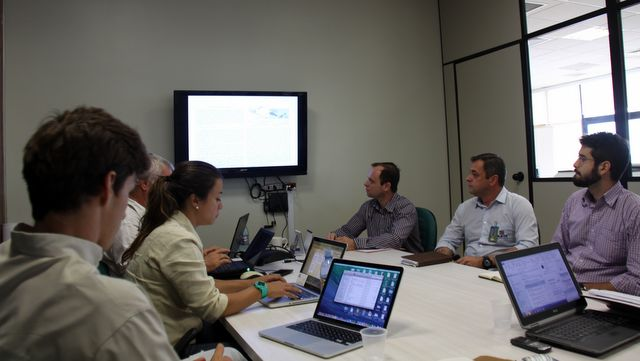
\includegraphics[width=0.85\textwidth]{Fotos/img_4836.jpg}
\caption{Reunião com Rijeza e ESBR.}
\end{figure}

Posteriormente, visitamos as instalações da Rijeza dentro da Usina para presenciar o funcionamento do robô que executa o hardcoating, assim como 
o estado das pás onde o hardcoating ja havia sido aplicado. 

\begin{figure}[H]
\centering
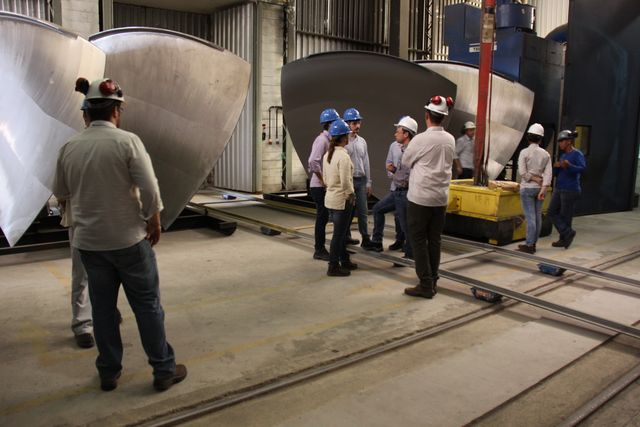
\includegraphics[width=0.85\textwidth]{Fotos/img_4881.jpg}
\caption{Equipe visita o galpão da Rijeza.}
\end{figure}
\begin{figure}[H]
\centering
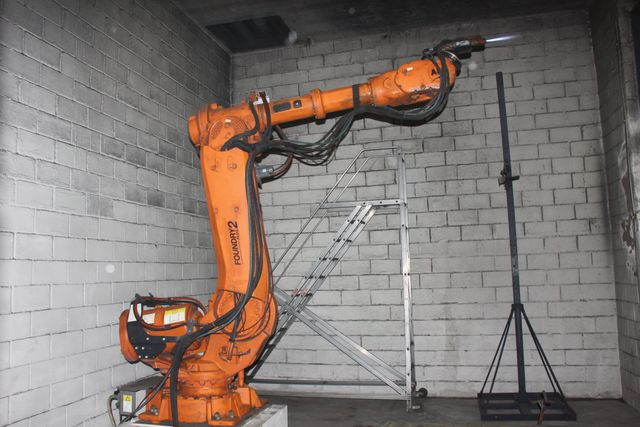
\includegraphics[width=0.85\textwidth]{Fotos/img_4858.jpg}
\caption{Instalações da Rijeza: Robô Industrial utilizado para
aplicação de hardcoating.}
\end{figure}
\begin{figure}[H]
\centering
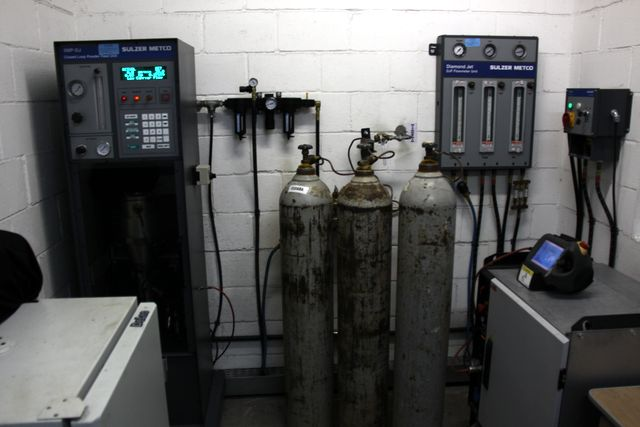
\includegraphics[width=0.85\textwidth]{Fotos/img_4850.jpg}
\caption{Instalações da Rijeza: secador, dosador, cilindros de gases, medidores,
unidade de segurança e o console do robô.}
\end{figure}
\begin{figure}[H]
\centering
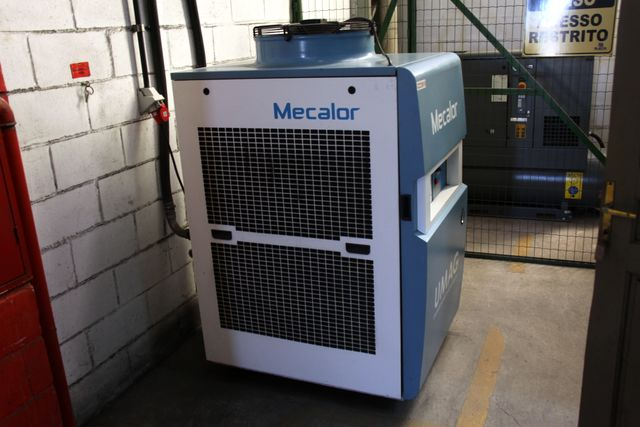
\includegraphics[width=0.85\textwidth]{Fotos/img_4852.jpg}
\caption{Instalações da Rijeza: cooler e compressor ao fundo.}
\end{figure}
\begin{figure}[H]
\centering
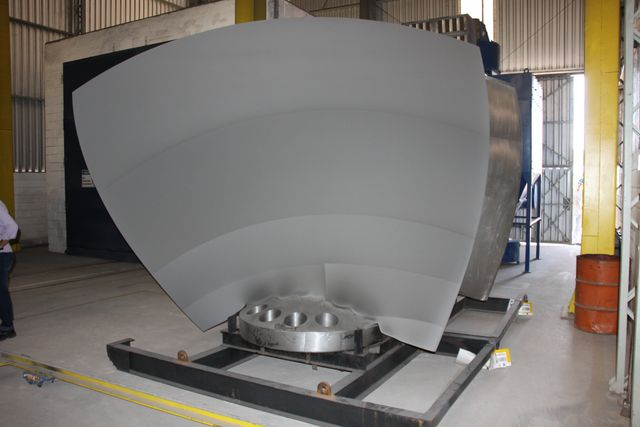
\includegraphics[width=0.85\textwidth]{Fotos/img_4886.jpg}
\caption{Pá já com Hardcoating aplicado.}
\end{figure}

Na parte da tarde visitamos uma unidade geradora para nos familiarizar com o
espaço onde a aplicação de hardcoating será feita, nosso objetivo foi inspecionar os locais 
de acesso, a montagem dos andaimes e a geometria da hélice.

\begin{figure}[H]
\centering
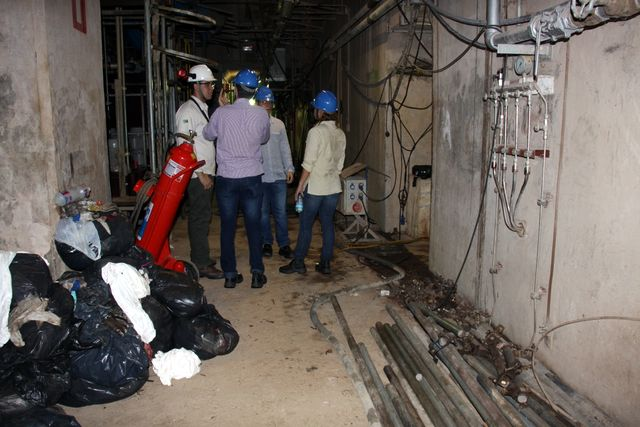
\includegraphics[width=0.85\textwidth]{Fotos/img_4905.jpg}
\caption{Corredor de acesso unidade geradora.}
\end{figure}

\begin{figure}[H]
\centering
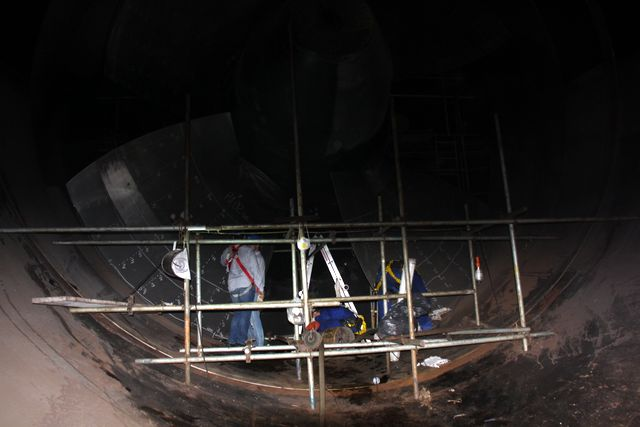
\includegraphics[width=0.85\textwidth]{Fotos/img_4931.jpg}
\caption{Montagem de andaimes dentro da unidade geradora.}
\end{figure}

\begin{figure}[H]
\centering
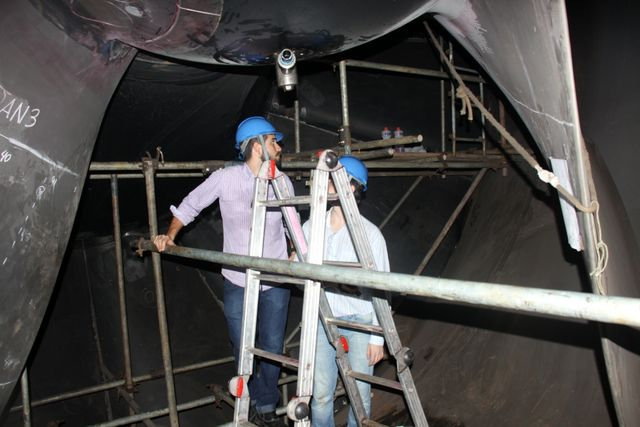
\includegraphics[width=0.85\textwidth]{Fotos/img_4966.jpg}
\caption{Engenheiros medem hélices.}
\end{figure}

\begin{figure}[H]
\centering
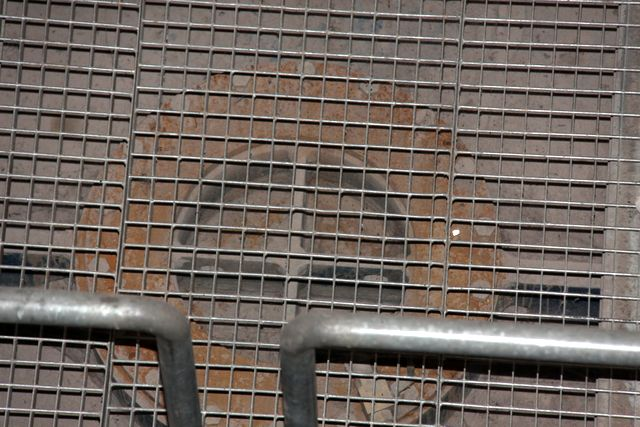
\includegraphics[width=0.85\textwidth]{Fotos/img_4978.jpg}
\caption{Em detalhe a escoltilha de acesso superior.}
\end{figure}

O segundo dia em Jirau foi voltado para a formulação dos conceitos possíveis
para o Robô EMMA. Em um primeiro momento avaliamos os braços mecânicos
disponíveis no mercado e todas suas possíveis aplicações no espaço da unidade gerador onde a inspeção deve acontecer.

\end{document}
